\section{Local polynomial fields}\label{sec:partII-A}

The polynomial labels of Definition~\ref{def:D07} prescribe continuum Taylor coefficients, whereas the Wilson measure integrates functions of group-valued links. Local sections connect the two: polynomials in the real and imaginary parts of finitely many link entries whose expansion on smooth test configurations reproduces a prescribed label. They initialize the renormalized insertions of Definition~\ref{def:D08}, hence the Wilson family of Theorem~\ref{thm:B}.

To build them we recover the connection jet from finitely many transported plaquette curvatures, whose linearizations are unit-square circulations (Section~\ref{sec:A-sections}); each curvature factor costs one power of the small-field threshold (Section~\ref{sec:A-bounds}). For the equation projections of Section~\ref{sec:partII-E}, Section~\ref{sec:A-equations} constructs auxiliary sections whose regraded equation labels $\mathsf R_d(\mathcal I_d)$ have exactly vanishing moments against distant observables. Section~\ref{sec:A-example} follows the curvature square through these constructions.

The lemmas of this section use only Part~I; the idea paragraph and Section~\ref{sec:A-example} also cite later results for illustration. The gauge metric and the Wilson measure of Definitions~\ref{def:D01}--\ref{def:D02} fix the measurements and the one-link integration by parts, Definition~\ref{def:D07} supplies the labels, and the derivative seminorm of Definition~\ref{def:D05a} measures the bounds. The sections are chosen once for each degree, and all constants of this section are fixed before the lattice volume and the stage block ratios, in the order of Section~\ref{sec:constants}.

\subsection{Labels, test holonomies and the Taylor map}\label{sec:A-labels}

Write $\mathcal J_j$ for the real space of the components $\mathcal A_j$ in Definition~\ref{def:D07}, the homogeneous radial potentials of degree~$j+1$. Every label in~$V_d$ is a polynomial on the finite-dimensional space
\begin{equation*}
\mathcal J_{\le d}=\bigoplus_{j+2\le d}\mathcal J_j\,.
\end{equation*}
Radial gauge and Euler's identity give $(j+2)\mathcal A_{j,a}(x)=\sum_bx^bF^{(j)}_{ba}(x)$, with $F^{(j)}$ the degree-$j$ part of the curvature; so a coordinate of~$\mathcal A_j$ has weight~$j+2$, two for the curvature and one for each derivative, and only finitely many monomials have weight at most~$d$. Adjoint action and conjugation preserve both gradings. Real and imaginary parts span each invariant component over~$\C$, giving bihomogeneous bases as in Definition~\ref{def:D07}. Conjugation in this real basis is coefficientwise and agrees with conjugation of polynomial values on real jets. Write $k_i$ for the number of jet-coordinate factors in~$b_{d,i}$. We identify a coefficient vector with its polynomial:
\begin{equation*}
\mathbf c(\mathsf j)=\sum_i c_i b_{d,i}(\mathsf j),\qquad b_{d,0}=\mathbf1\,.
\end{equation*}

We evaluate lattice observables on the test holonomies~\eqref{eq:I12-test-holonomy}, on the lattice~$\Z^4$ covering the torus. With $\mathcal A^{\le d}=\sum_{j+2\le d}\mathcal A_j$, they are
\begin{equation}\label{eq:A-holonomy}
U(h_{\rm lat},\mathsf j)(x,a)=u(1),\qquad
u'(s)=u(s)\,h_{\rm lat}\mathcal A_a^{\le d}(h_{\rm lat}(x+se_a)),\qquad u(0)=1\,.
\end{equation}
This linear equation with continuous $\g$-valued coefficients has a unique global solution~\cite[Theorem~3.9]{Teschl2012}. It lies in the closed group~$G$, being a uniform limit of products of exponentials of elements of~$\g$ by Gronwall's inequality~\cite[Lemma~2.7]{Teschl2012}, and its Volterra series shows that it depends smoothly on $(h_{\rm lat},\mathsf j)$. Homogeneity and uniqueness give
\begin{equation}\label{eq:A-dilation}
U(h_{\rm lat},\mathsf j)=U(1,\operatorname{sc}_{h_{\rm lat}}\mathsf j),\qquad
\operatorname{sc}_{h_{\rm lat}}\mathsf j=(h_{\rm lat}^{j+2}\mathcal A_j)_j,\qquad U(0,\mathsf j)=1\,.
\end{equation}

The Taylor map of Section~\ref{sec:local-fields} reads off the continuum polynomial seen by a lattice observable. Recall that, for a smooth function~$O$ of finitely many cover links, $\taylormap_{d}O$ is the Taylor polynomial at zero of $\mathsf j\mapsto O(U(1,\mathsf j))$ on~$\mathcal J_{\le d}$, with the monomials of weight above~$d$ discarded. By~\eqref{eq:A-dilation}, a monomial of weight~$w$ contributes $h_{\rm lat}^w$ to $O(U(h_{\rm lat},\mathsf j))$. Hence the derivatives of $O(U(h_{\rm lat},\mathsf j))$ at $h_{\rm lat}=0$ through order~$d$ are those of $\mathbf c(\operatorname{sc}_{h_{\rm lat}}\mathsf j)$ for every jet, where $\mathbf c\in V_d$, exactly when $\taylormap_{d}O=\mathbf c$. A local section, constructed below, is a right inverse of the Taylor map, linear in the label: this is the sense of the word \emph{section}.

For a cover plaquette~$\square$ based at~$z$ and a path~$\gamma$ from~$0$ to~$z$, write $U_\gamma$ for the ordered product of successive oriented links, read from the initial point to the endpoint. Define the transported curvature (Figure~\ref{fig:A-transported}) by
\begin{equation*}
\sigma_{\gamma,\square}(U)=\operatorname{Ad}(U_\gamma)F_\square(U),\qquad
F_\square(U)=\operatorname{proj}_{\g}\frac{U_\square-U_\square^{-1}}2\,.
\end{equation*}
The projection is orthogonal for the normalized Frobenius metric of Definition~\ref{def:D01}. These measurements transform by the adjoint action at~$0$. They are real polynomial functions of the real and imaginary parts of link entries, since $U_e^{-1}=U_e^*$.

\begin{figure}[ht]
\centering
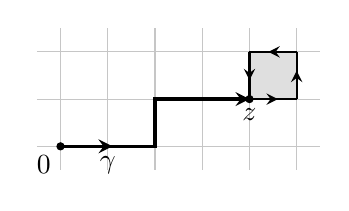
\begin{tikzpicture}[scale=0.6,>=stealth]
\draw[gray!45] (-0.5,-0.5) grid (5.5,2.5);
\fill[gray!25] (4,1) rectangle (5,2);
\draw[thick,->] (4,1)--(4.6,1); \draw[thick] (4.5,1)--(5,1);
\draw[thick,->] (5,1)--(5,1.6); \draw[thick] (5,1.5)--(5,2);
\draw[thick,->] (5,2)--(4.4,2); \draw[thick] (4.5,2)--(4,2);
\draw[thick,->] (4,2)--(4,1.4); \draw[thick] (4,1.5)--(4,1);
\node at (4.5,1.5) {$\square$};
\draw[very thick,->] (0,0)--(1.1,0); \draw[very thick] (1,0)--(2,0)--(2,1)--(3.1,1); \draw[very thick,->] (3,1)--(4,1);
\node[below] at (1,0) {$\gamma$};
\fill (0,0) circle (2.5pt) node[below left] {$0$};
\fill (4,1) circle (2.5pt) node[below] {$z$};
\end{tikzpicture}
\caption{A transported curvature $\sigma_{\gamma,\square}=\operatorname{Ad}(U_\gamma)F_\square(U)$, drawn in one coordinate plane: the curvature of the plaquette~$\square$ based at~$z$ is carried to the origin along the lattice path~$\gamma$.}\label{fig:A-transported}
\end{figure}

\subsection{Taylor-normalized sections}\label{sec:A-sections}

\begin{definition}[Local sections]\label{def:D19}
For a finite site stencil $\Sigma_d\subset\Z^4$, a local section has the form
\begin{equation*}
\localsection{d}[\mathbf c](U)=
\sum_{\nu,\mu}p_{\nu\mu}^{(d)}(\mathbf c)
\prod_{e,\alpha,\delta}U_e(\alpha,\delta)^{\nu_{e\alpha\delta}}\overline{U_e(\alpha,\delta)}^{\mu_{e\alpha\delta}}\,.
\end{equation*}
The product uses positive links with both endpoints in~$\Sigma_d$ and matrix indices $1\le\alpha,\delta\le n_G$. The sum is finite over nonnegative multi-indices; each coefficient is complex linear in~$\mathbf c$. The construction below chooses such a map to represent each continuum label.
\end{definition}

For a torus of side~$n_{\rm tor}$ (the side~$s$ of Definition~\ref{def:D02}), write $[x]$ for reduction of $x\in\Z^4$ modulo~$n_{\rm tor}$. Placement at a torus site~$y$ means evaluation on the periodic extension $U^{[y]}(x,a)=U(y+[x],a)$; denote it by $\localsection{d}[\mathbf c](y;U)$. On the cover, $\localsection{d}[\mathbf c](0;U)=\localsection{d}[\mathbf c](U)$. For $h\in\hypercubic$, define the configuration and jet actions by
\begin{align*}
(h^*U)(x,a)&=
\begin{cases}U(hx,b),&he_a=e_b,\\ U(hx-e_b,b)^{-1},&he_a=-e_b,\end{cases}\\
(h\mathsf j)_{j,a}(z)&=\sum_bh_{ab}\mathcal A_{j,b}(h^{-1}z),\qquad
(h\mathbf c)(\mathsf j)=\mathbf c(h^{-1}\mathsf j)\,.
\end{align*}
This action preserves homogeneity and radial gauge. Reality and covariance mean
\begin{equation*}
\localsection{d}[\overline{\mathbf c}](U)=\overline{\localsection{d}[\mathbf c](U)},\qquad
\localsection{d}[\mathbf c](h^*U)=\localsection{d}[h\mathbf c](U)\quad(h\in\hypercubic),
\end{equation*}
with conjugation as fixed above.

The following result supplies the sections specified in Section~\ref{sec:local-fields}; the unit normalization is exact at every configuration.
\begin{lemma}[Taylor-normalized sections]\label{lem:A1}
For every~$d$, a box stencil $\Sigma_d=[-\varrho_d,\varrho_d]^4\cap\Z^4$ and sections can be chosen gauge invariant, real and $\hypercubic$ covariant, with $\localsection{d}[\mathbf1]=1$, so that, for every $\mathbf c\in V_d$, radial jet~$\mathsf j$ and $0\le q\le d$,
\begin{equation}\label{eq:A-Taylor}
\left.\frac{d^q}{dh_{\rm lat}^q}\localsection{d}[\mathbf c](U(h_{\rm lat},\mathsf j))\right|_{h_{\rm lat}=0}
=\left.\frac{d^q}{dh_{\rm lat}^q}\mathbf c(\operatorname{sc}_{h_{\rm lat}}\mathsf j)\right|_{h_{\rm lat}=0}\,.
\end{equation}
\end{lemma}
Equivalently, $\taylormap_{d}\localsection{d}[\mathbf c]=\mathbf c$ for every $\mathbf c\in V_d$. The identity imposes no equality at positive spacing, and no compatibility between $\localsection{d}$ and $\localsection{d+1}$ is required. We fix the sections constructed in the following proof.

\begin{proof}
There are three steps: finitely many curvature measurements determine the truncated jet; an equivariant polynomial inverse of these measurements, composed with the label, gives a section with the right Taylor map; averaging over~$\hypercubic$ gives covariance and a common stencil. If $d<2$, the labels are constant and their constant sections suffice. Fix $d\ge2$.

\emph{Step 1: Curvatures determine the truncated jet.} The measurements $\sigma_{\gamma,\square}(U(1,\mathsf j))$ are smooth in~$\mathsf j$, and all links equal~$1$ at $\mathsf j=0$. The first variation of a link solution is the edge integral of the potential; that of a plaquette measurement is the circulation of the potential around the plaquette. Transport along~$\gamma$ contributes nothing at first order, because $F_\square(1)=0$. By the fundamental theorem of calculus on each edge, the circulation around the unit square at~$x$ in the plane of the axes $a<b$ is
\begin{equation*}
N_{ab}(x)=\int_0^1\!\int_0^1
(\partial_a\mathcal A_b-\partial_b\mathcal A_a)(x+\xi e_a+\eta e_b)\,d\xi\,d\eta\,.
\end{equation*}
Suppose all these linearized measurements vanish at $\mathcal A=\sum_{j=0}^{j_*}\mathcal A_j$. Then the polynomial~$N_{ab}$ vanishes on~$\Z^4$, hence identically: a polynomial vanishing on~$\Z^4$ is zero, by induction on the number of variables. The averaging shifts only lower the degree, so the homogeneous part of~$N_{ab}$ of degree~$j_*$ is $(\partial_a\mathcal A_{j_*,b}-\partial_b\mathcal A_{j_*,a})(x)$. It vanishes, and antisymmetry covers the other ordered pairs. Differentiating the radial condition and using Euler's identity gives
\begin{equation*}
(j_*+2)\mathcal A_{j_*,b}(z)=\sum_a z^a(\partial_a\mathcal A_{j_*,b}-\partial_b\mathcal A_{j_*,a})(z)=0\,.
\end{equation*}
Remove this component and descend in~$j_*$: the common kernel is zero. Adding a measurement whenever the kernel is nonzero decreases its dimension, so finitely many measurements $\sigma_1,\ldots,\sigma_{M_{\rm meas}}$ give a joint map
\begin{equation*}
\mathsf S:\mathcal J_{\le d}\longrightarrow\g^{M_{\rm meas}},\qquad
\mathsf S(\mathsf j)=(\sigma_l(U(1,\mathsf j)))_{l=1}^{M_{\rm meas}}
\end{equation*}
with injective derivative~$D\mathsf S(0)$.

\emph{Step 2: A polynomial inverse to the required order.} By uniqueness of the link equation, a constant gauge transformation $v\in G$ takes the test links of~$\mathsf j$ to those of~$\operatorname{Ad}(v)\mathsf j$, so~$\mathsf S$ is adjoint equivariant. The range of $D\mathsf S(0)$ is invariant; composing the inverse of $D\mathsf S(0)$ on it with orthogonal projection onto it gives an equivariant linear map $C:\g^{M_{\rm meas}}\to\mathcal J_{\le d}$ with $CD\mathsf S(0)=I$. By the inverse function theorem~\cite[Theorem~9.24]{Rudin1976}, $C\mathsf S$ has a local inverse~$\varphi$ near zero, smooth by differentiating $D\varphi=(D(C\mathsf S)\circ\varphi)^{-1}$. The adjoint actions are isometric, so $\varphi$ can be taken on invariant balls, where injectivity of~$C\mathsf S$ makes it equivariant. Put $f=\varphi\circ C$. Near zero, $f\mathsf S(\mathsf j)=\mathsf j$, $f(0)=0$ and $f(\operatorname{Ad}(v)z)=\operatorname{Ad}(v)f(z)$ for $v\in G$. Consequently the Taylor polynomial $T_df(z)=\sum_{k=1}^{d}D^kf(0)[z,\ldots,z]/k!$ is adjoint equivariant and has no constant term. Define
\begin{equation*}
Q_i(z)=b_{d,i}(T_df(z)),\qquad
\Psi_{\mathbf c}(U)=\sum_i c_iQ_i(\sigma_1(U),\ldots,\sigma_{M_{\rm meas}}(U))\,.
\end{equation*}
The polynomials~$Q_i$ are invariant and real on real arguments, and $Q_0=1$. If $b_{d,i}$ has factor count~$k_i$, every monomial of~$Q_i$ has at least~$k_i$ factors. Taylor's formula gives $T_df(\mathsf S(\mathsf j))=\mathsf j+O(|\mathsf j|^{d+1})$ near zero, hence
\begin{equation*}
\Psi_{\mathbf c}(U(1,\mathsf j))=\mathbf c(\mathsf j)+O_{\mathbf c}(|\mathsf j|^{d+1}),\qquad
\taylormap_{d}\Psi_{\mathbf c}=\mathbf c\,.
\end{equation*}
The polynomial~$Q_i$ itself need not have degree at most~$d$ in the curvature measurements.

\emph{Step 3: Covariance and a common stencil.} Average the section by
\begin{equation}\label{eq:A-average}
\localsection{d}[\mathbf c](U)=\frac1{|\hypercubic|}
\sum_{h\in\hypercubic}\Psi_{h^{-1}\mathbf c}(h^*U)\,.
\end{equation}
Changing the summation variable to $h'h$ proves $\localsection{d}[\mathbf c](h'^*U)=\localsection{d}[h'\mathbf c](U)$. Simultaneous adjoint covariance of the measurements gives gauge invariance. The real basis and the signed-permutation action give reality; the constant column remains one. The action preserves factor count, so averaging retains the lower bound on the number of curvature factors.

For a positive image direction, the pulled-back link equation has the coefficient of~$h^{-1}\mathsf j$, namely $h_{\rm lat}\sum_bh_{ba}\mathcal A_b^{\le d}(h_{\rm lat}h(x+se_a))$. Reversing the parameter and inverting the transport covers a negative image direction. Uniqueness gives $h^*U(h_{\rm lat},\mathsf j)=U(h_{\rm lat},h^{-1}\mathsf j)$. Each term of~\eqref{eq:A-average} therefore has Taylor map~$\mathbf c$. A signed image of a transported curvature is again a transported curvature, up to sign: reversal changes $F_\square$ to $-F_\square$, and a change of base point gives conjugation by the intervening boundary transport. Enclose the finitely many resulting paths and plaquettes in a box $\Sigma_d=[-\varrho_d,\varrho_d]^4\cap\Z^4$. This stencil contains zero and is signed-permutation invariant. Expanding the finite polynomial in matrix entries gives Definition~\ref{def:D19}. This proves~\eqref{eq:A-Taylor}, which is~\eqref{eq:I12-section-Taylor}.
\end{proof}

\subsection{Small-field bounds}\label{sec:A-bounds}

We bound normalized initial insertions using the ordered left derivatives of Definition~\ref{def:D05a}. At a placement~$y$, set $Y=y+[\Sigma_d]$; being healthy on~$Y$ means that every plaquette meeting~$Y$ has chord at most~$t$. A direction is permitted when
\begin{equation*}
|\dot{\mathcal A}_e|\le t(1+\operatorname{dist}(e^-,y))^\varpi\,.
\end{equation*}
Here $[\Sigma_d]$ is the torus image of the stencil, and $\operatorname{dist}(x,y)=\min_{z\in n_{\rm tor}\Z^4}|\tilde x-\tilde y+z|_\infty$ is the periodic maximum-coordinate distance, for any lifts $\tilde x,\tilde y$.
\begin{lemma}[Section bounds]\label{lem:A-bounds}
Each basis column is a polynomial in transported curvatures with at least~$k_i$ factors per monomial. For all $d,k,\varpi\in\N$ there are finite constants $C_{d,k,\varpi}$ and $C_d$ such that, on every torus, for every placement~$y$, $0<t\le1$, configuration healthy on~$Y$, and permitted direction list of length $q\le k$,
\begin{equation}\label{eq:A-section-bound}
\bigl|D^L_{\dot{\mathcal A}_1}\cdots D^L_{\dot{\mathcal A}_q}
\localsection{d}[b_{d,i}](y;U)\bigr|\le C_{d,k,\varpi}t^{k_i}\,.
\end{equation}
For arbitrary configurations,
\begin{equation}\label{eq:A-global-bound}
\sup_{i,y,U}|\localsection{d}[b_{d,i}](y;U)|\le C_d\,.
\end{equation}
\end{lemma}
Each curvature factor is at most of the size~$t$ of the plaquettes it reads, so a column with $k_i$ factors is of order~$t^{k_i}$ on healthy configurations. The proof uses the curvature polynomials constructed in Lemma~\ref{lem:A1}.
\begin{proof}
First note that $|F_\square(U)|\le\chord(U_\square)$: orthogonal projection is contractive and $\|U_\square-U_\square^*\|_{\rm F}\le2\|U_\square-1\|_{\rm F}$. Adjoint transport is isometric, so an undifferentiated curvature measurement is bounded by~$t$. An order-$q$ left derivative of a fixed path product is a finite sum of products of unitary matrices and exactly~$q$ direction matrices. On the fixed stencil their norms are at most a constant times~$t$, since periodic distance is bounded by cover distance. Thus each differentiated measurement is $O(t^q)$, and hence $O(t)$ when $q\ge1$. This argument also applies when cover links coincide after placement: one first differentiates the cover expression and then assigns the same direction to coincident links.

Apply the product rule to the curvature polynomials of~\eqref{eq:A-average}. Every differentiated monomial still has at least~$k_i$ factors, each bounded by a constant times~$t$. There are finitely many terms; since $t\le1$, their sum gives~\eqref{eq:A-section-bound}, including order zero. Each entry of a unitary matrix has absolute value at most one, so the finite matrix-entry polynomial gives~\eqref{eq:A-global-bound}. The formula also gives smoothness, measurability and locality. The constants depend on the sections, $G,d,k,\varpi$ as applicable, and finite maxima make them nondecreasing in the integer parameters. They are fixed before the stage block ratios in Section~\ref{sec:constants}.
\end{proof}

By linearity, Lemma~\ref{lem:A-bounds} bounds permitted derivatives of $\localsection{d}[t^{-\factorcount}\mathbf c]$ by $C_{d,k,\varpi}\sum_i|c_i|$ on the healthy set: the factor $t^{-k_i}$ cancels $t^{k_i}$. Taking $t=t_N$, $k=\mathfrak q_{J_N}$ and $\varpi=\varpi_{J_N}$ bounds the initial marked density of~\eqref{eq:I12-marked-evolution} on the healthy set, in the sense of Definition~\ref{def:D05a}. On unhealthy configurations the global bound gives $C_d\sum_i|c_i|t^{-k_i}$; the proof of Lemma~\ref{lem:E2.1} places this contribution in a merged forced remainder of~\eqref{eq:I12-marked-representation}.

\subsection{Auxiliary equation sections}\label{sec:A-equations}

Exact lattice equation identities require different sections, still polynomial and local with the same small-field bounds. On~$\mathcal J_j$ define the Maxwell subspace and the equation labels by
\begin{equation*}
\mathcal J_j^{\rm Max}=\Bigl\{\mathcal A_j:\ \sum_a\partial_a(\partial_a\mathcal A_{j,b}-\partial_b\mathcal A_{j,a})=0\ \text{for every }b\Bigr\},\qquad
\mathcal I_d=\Bigl\{p\in V_d:p|_{\prod_j\mathcal J_j^{\rm Max}}=0\Bigr\}\,.
\end{equation*}
Here restriction uses only $j+2\le d$. Substitution into $\prod_j\mathcal J_j^{\rm Max}$ preserves bidegree, so $\mathcal I_d$ is the direct sum of its bihomogeneous parts. Order bidegrees~$(w,k)$ by the lexicographic order of~$(k,w)$. A triangular regrading (a unipotent change of labels) is a complex-linear map on~$V_d$ whose difference from the identity sends each bihomogeneous polynomial into strictly later bidegrees. There are finitely many bidegrees, so this difference is nilpotent and the map is invertible; the map and its inverse preserve the filtration by minimum factor count.

\paragraph{Idea: free equations in an interacting theory.} Haar integration by parts in one link, a lattice Schwinger--Dyson identity, shows that for $\beta\ne0$ the force~$\mathcal E_e$ of~\eqref{eq:A-link-equation}, the derivative of the Wilson energy in the link~$e$, has zero moments when multiplied by a function independent of~$U_e$ and by observables of distant links. Its linearization is the divergence of the linearized curvature, and the Maxwell equations enter only through this linearization. An equation label is a sum of products with one factor vanishing on Maxwell jets. Replacing that factor by forces and the others by curvature measurements gives an observable with exactly vanishing exterior moments, whose Taylor map is the label plus later terms, produced by the higher-weight linear terms of the lattice force and by nonlinear corrections. The construction therefore exhibits exact lattice equations for the labels in~$\mathsf R_d(\mathcal I_d)$: this is the lattice form of the vanishing of equation-of-motion operators at separated points. For example, put $F_{ab}=\partial_a\mathcal A_{0,b}-\partial_b\mathcal A_{0,a}$ and $(\partial\cdot F)_b=\sum_c\partial_c(\partial_c\mathcal A_{1,b}-\partial_b\mathcal A_{1,c})$, both constant. The label $q_{\rm eq}=\sum_b\langle(\partial\cdot F)_b,(\partial\cdot F)_b\rangle_\g$ lies in~$\mathcal I_6$ and has bidegree $(6,2)$. The only later bidegree of weight at most six is~$(6,3)$, so $\mathsf R_6q_{\rm eq}-q_{\rm eq}$ is a cubic invariant polynomial in the~$F_{ab}$; nothing below requires it to vanish. The equation count is shared with the free theory, the separated correlations are not: Proposition~\ref{prop:FC} and~\eqref{eq:E-equation-count} give $\dim\nullspace{d}(S)=\dim\mathcal I_d$, while in the selected phase $\tracetwopoint$ is asymptotic to $\traceamplitude r^{-8}\log^{-2}(1/r)$ (Theorem~\ref{prop:TR}), and on no interval $(0,\delta)$ does $\tracetwopoint$ agree with a finite Wick profile (Proposition~\ref{prop:NF}).

\paragraph{Lattice symmetries.} We record the symmetries of the Wilson measure deferred from Definition~\ref{def:D02}. A site gauge transformation acts on plaquette holonomies by conjugation, and an affine isometry $h_{\rm iso}(x)=hx+b$ with $h\in\hypercubic$ by conjugation, possibly after inversion; both preserve~$\wilsonterm$. Product probability Haar measure is invariant under fixed left and right multiplication, inversion and permutation~\cite[Corollary~2.28 and Proposition~2.31]{Folland2015}. Hence, for every integer side $n_{\rm tor}\ge1$, real~$\beta$, site gauge transformation~$\gamma_{\rm g}$ and bounded measurable~$F$,
\begin{equation}\label{eq:A-Wilson-invariance}
\int F(U^{\gamma_{\rm g}})\,d\mu_{n_{\rm tor},\beta}(U)
=\int F(h_{\rm iso}^*U)\,d\mu_{n_{\rm tor},\beta}(U)
=\int F(U)\,d\mu_{n_{\rm tor},\beta}(U)\,.
\end{equation}

For a torus site~$y$, put $\mathbb B_r(y)=\{x:\operatorname{dist}(x,y)\le r\}$. An exterior spectator outside~$\mathbb B_r(y)$ is a bounded measurable function of the positive links having both endpoints outside~$\mathbb B_r(y)$; it need not be gauge invariant. The following identity supplies the auxiliary equation observables used in Section~\ref{sec:partII-E}.
\begin{lemma}[Auxiliary equation sections]\label{lem:A-R4}
For every~$d$ there are a local section~$V_d^{\rm aux}$ as in Definition~\ref{def:D19}, an invertible triangular regrading~$\mathsf R_d$ of~$V_d$, and $r_d,M_d\in\N$ with the following properties.
\begin{enumerate}[label=\textup{(\roman*)},nosep]
\item The section has its own box stencil, is gauge invariant, real and $\hypercubic$ covariant, satisfies $V_d^{\rm aux}[\mathbf1]=1$ and~\eqref{eq:A-Taylor}, and satisfies \eqref{eq:A-section-bound}--\eqref{eq:A-global-bound} with its own constants.
\item The map~$\mathsf R_d$ fixes~$\mathbf1$ and commutes with conjugation and~$\hypercubic$.
\item For every $n_{\rm tor}\ge M_d$, $\beta\ne0$, placement~$y$, $p\in\mathcal I_d$ and exterior spectator~$F_{\rm ext}$ outside~$\mathbb B_{r_d}(y)$,
\begin{equation}\label{eq:A-aux-zero}
\int V_d^{\rm aux}[\mathsf R_dp](y;U)F_{\rm ext}(U)\,d\mu_{n_{\rm tor},\beta}(U)=0\,.
\end{equation}
\end{enumerate}
\end{lemma}
The exact-equation subspace $\mathsf R_d(\mathcal I_d)$ is compared with the selected primary family in Section~\ref{sec:partII-E}. All choices in the following proof depend only on~$G,d$ and the label basis.

\begin{proof}
There are three steps: one-link integration by parts gives zero moments; forces realize every linear functional vanishing on Maxwell jets; products of forces and curvature measurements, averaged, represent equation labels up to a triangular regrading, which is then inverted.

\emph{Step 1: One-link equations.} Extend the curvature $F_\square$ of Section~\ref{sec:A-labels} to $F_{ab}(U;x)$ for ordered axes by antisymmetry, with $F_{aa}=0$. For a positive link $e=(x,a)$ set
\begin{equation*}
\mathcal E_e(U)=\sum_{b\ne a}\left(F_{ab}(U;x)-\operatorname{Ad}(U(x-e_b,b)^{-1})F_{ab}(U;x-e_b)\right)\,.
\end{equation*}
On a torus of side at least two, direct differentiation gives
\begin{equation}\label{eq:A-link-equation}
D^L_{e,A}E^{\rm W}(U)=\langle A,\mathcal E_e(U)\rangle_{\g}\,.
\end{equation}
Indeed, the forward plaquette contributes $-n_G^{-1}\operatorname{Re}\tr(AU_\square)=\langle A,F_\square\rangle_{\g}$. The backward plaquette, rebased at~$x$, contributes the negative of the transported curvature in the display. These are the two incidences for each transverse axis; antisymmetry gives the signs for the opposite ordering.

If a continuous multiplier~$g$ is independent of~$U_e$, and a bounded measurable~$F_{\rm ext}$ is also independent of~$U_e$, left invariance of Haar measure gives
\begin{equation*}
0=\left.\frac{d}{d\epsilon}\int g(U)F_{\rm ext}(U)e^{-\beta E^{\rm W}(U^{e,A,\epsilon})}\,dU\right|_{\epsilon=0}
=-\beta Z_{n_{\rm tor},\beta}\int\langle A,\mathcal E_e\rangle_{\g}gF_{\rm ext}\,d\mu_{n_{\rm tor},\beta}\,.
\end{equation*}
Here $U^{e,A,\epsilon}_e=e^{\epsilon A}U_e$ and all other links are fixed. Compactness bounds the derivative of the smooth density uniformly, justifying differentiation even for measurable~$F_{\rm ext}$.

Choose a path~$\gamma_e$ from~$0$ to~$e^-$ avoiding~$e$. If~$g$ also avoids~$e$, then
\begin{equation*}
\Upsilon_{e,\xi}(U)=\langle \xi,\operatorname{Ad}(U_{\gamma_e})\mathcal E_e(U)\rangle_{\g}g(U)
\end{equation*}
has zero moment for every $\xi\in\g$ against every exterior spectator. To see this, expand $\operatorname{Ad}(U_{\gamma_e}^{-1})\xi$ in a fixed orthonormal basis of~$\g$ and apply the preceding identity to each coefficient times~$gF_{\rm ext}$. These multipliers are independent of~$U_e$. There is one radius and one minimum torus side for any finite collection of such expressions: enlarge the radius to contain both endpoints of every varied link, and the side until distinct links in their finite cover supports remain distinct after wrapping. The same choices work at every placement.

\emph{Step 2: Enough measurements with avoidance.} Any path can avoid one specified link: replace a traversal of that link by three sides of a square in a transverse direction. For each plaquette orientation only finitely many base points give a plaquette containing that link. Removing these points does not affect Step~1 of the proof of Lemma~\ref{lem:A1}: if a polynomial vanishes at all but finitely many points of~$\Z^4$, its restriction to each coordinate line through an integer point has infinitely many zeros, so it vanishes on~$\Z^4$ and hence identically. Thus curvature measurements whose paths and plaquettes avoid~$e$ still have injective joint linearization. Finite-dimensional duality therefore realizes every linear functional on~$\mathcal J_{\le d}$ by finitely many components.

For every linear functional~$\ell$ on~$\mathcal J_j$ vanishing on~$\mathcal J_j^{\rm Max}$, a finite combination of force linearizations equals $\mathsf j\mapsto\ell(\mathcal A_j)$ on $\mathcal J_{\le j+2}=\bigoplus_{i\le j}\mathcal J_i$. To see this, extend the circulations~$N_{ab}$ of Step~1 of the proof of Lemma~\ref{lem:A1} antisymmetrically. The force linearization at~$e=(x,a)$ is
\begin{equation*}
L_a(\mathsf j;x)=\sum_b\bigl(N_{ab}(x)-N_{ab}(x-e_b)\bigr)\,.
\end{equation*}
Suppose that every $L_a(\mathsf j;x)$, $x\in\Z^4$, vanishes for a jet $\mathcal A=\sum_{i\le j_*}\mathcal A_i$. Each $L_a(\mathsf j;\cdot)$ is a polynomial, hence zero. In $N_{ab}(x)-N_{ab}(x-e_b)$ a component~$\mathcal A_i$ contributes a polynomial of degree at most~$i-1$, and $\mathcal A_{j_*}$ contributes $\partial_b(\partial_a\mathcal A_{j_*,b}-\partial_b\mathcal A_{j_*,a})(x)$ plus terms of lower degree. The part of degree~$j_*-1$ therefore gives $\sum_b\partial_b(\partial_a\mathcal A_{j_*,b}-\partial_b\mathcal A_{j_*,a})=0$, that is, $\mathcal A_{j_*}\in\mathcal J_{j_*}^{\rm Max}$. A functional of this top component annihilating~$\mathcal J_{j_*}^{\rm Max}$ therefore annihilates the common kernel of the force measurements. Finite-dimensional duality puts it in their linear span. Transport paths do not enter the linearization and can be chosen to avoid their varied links. On~$\mathcal J_{\le d}$ the same combination can have additional linear terms only at engineering weights above~$j_*+2$.

\emph{Step 3: Polynomial lifts and the triangular map.} Choose linear projections $\pi_j:\mathcal J_j\to\mathcal J_j^{\rm Max}$ and put $\pi=\prod_j\pi_j$. A polynomial belongs to~$\mathcal I_d$ precisely when $p\circ\pi=0$. For a product of linear coordinates,
\begin{equation*}
\prod_{i=1}^{k_{\rm tot}}\ell_i-\prod_{i=1}^{k_{\rm tot}}(\ell_i\circ\pi)
=\sum_{i=1}^{k_{\rm tot}}\left[\prod_{l<i}(\ell_l\circ\pi)\right]
(\ell_i-\ell_i\circ\pi)\prod_{l>i}\ell_l\,.
\end{equation*}
Consequently every bihomogeneous equation label is a finite sum of products with one linear factor vanishing on some~$\mathcal J_j^{\rm Max}$, with the same engineering weight and factor count. The individual factors need not be invariant. We use the Taylor map~$\taylormap_{d}$ of Section~\ref{sec:A-labels}; every coordinate has weight at least two. Call a lattice observable~$O$ a lift of a bihomogeneous polynomial~$q$ if $\taylormap_{d}O-q$ consists of monomials later than~$q$ in the $(k,w)$ order.

Lift the distinguished factor by a finite combination of transported forces from Step~2. For each summand, lift the other factors by curvature measurements avoiding its varied link, matching their full linear parts through engineering weight~$d$. The resulting expression has the zero-moment property of Step~1 and at least~$k_{\rm tot}$ curvature factors. Indeed, every force is a difference of two transported curvatures per transverse axis. The expression is a lift of the prescribed product: the additional linear terms of the force have greater engineering weight, and every nonlinear correction increases factor count. The square-measurement lifts have their prescribed full linear parts, so introduce only the latter kind of correction. Taylor polynomials exist by the smooth dependence of the test holonomies on the jet.

Average over constant gauge transformations. All factors transform by adjoint matrices at the origin, so the orbit lies in the finite-dimensional span of finitely many fixed-degree colour-coordinate monomials on the same measurements; each orbit function keeps zero moments, with colour vectors rotated by $\operatorname{Ad}(v^{-1})$. The Haar average is therefore a gauge-invariant finite combination of orbit functions; it keeps zero moments, minimum factor count and the lift property, and its Taylor map is invariant.

In each bidegree extend a basis of~$\mathcal I_d$ to a basis of the invariant label space in that bidegree, lifting the complementary vectors by Lemma~\ref{lem:A1}. Lift~$\mathbf1$ to~$1$, since $\mathcal I_d$ contains no nonzero constant. Summing gives a linear lift~$p\mapsto\mathcal Y_p$. Replace this lift by the two successive averages
\begin{align*}
\mathcal Y'_p(U)&=\frac1{|\hypercubic|}\sum_{h\in\hypercubic}\mathcal Y_{h^{-1}p}(h^*U),\\
\mathcal Y^{\rm sym}_p&=\frac12\left(\mathcal Y'_p+\overline{\mathcal Y'_{\bar p}}\right)\,.
\end{align*}
The Taylor map commutes with both operations. The real Maxwell equations and the chain rule make $\mathcal J_j^{\rm Max}$, and hence~$\mathcal I_d$, stable under signed permutations, adjoint transformations and conjugation. The zero-moment property survives the signed average by~\eqref{eq:A-Wilson-invariance}, changing the spectator by the inverse isometry; the exterior set is preserved. Conjugation uses~$\overline{F_{\rm ext}}$. A reversed varied link uses a right derivative of the Wilson energy, whose Haar identity is identical. Thus the averaged equation representatives remain finite sums of one-link action derivatives with link-independent multipliers and avoiding transport paths.

Let $\mathsf R_dp=\taylormap_{d}\mathcal Y^{\rm sym}_p$. Then $\mathsf R_d-I$ strictly raises~$(k,w)$. There are finitely many bidegrees of weight at most~$d$, so $(\mathsf R_d-I)^{n_0}=0$ for some integer~$n_0$, and
\begin{equation*}
\mathsf R_d^{-1}=\sum_{l=0}^{n_0-1}(-1)^l(\mathsf R_d-I)^l,\qquad
V_d^{\rm aux}[\mathbf c]=\mathcal Y^{\rm sym}_{\mathsf R_d^{-1}\mathbf c}\,.
\end{equation*}
This gives invertibility and Taylor normalization; the averages give the symmetry and unit identities. The inverse preserves minimum factor count, so Lemma~\ref{lem:A-bounds} applies to these sections with their own constants. A signed-invariant box enclosing all paths and plaquettes gives a common stencil. Take $r_d,M_d$ as maxima for an ideal basis; linearity gives~\eqref{eq:A-aux-zero}.
\end{proof}

\subsection{Example: the curvature square}\label{sec:A-example}

We follow one familiar observable through the construction. Sections~\ref{sec:partII-E} and~\ref{sec:partII-F} construct the terminal map and the quotient used at its end.

\paragraph{The label.} With $F_{ab}$ as in Section~\ref{sec:A-equations}, radial gauge gives $\mathcal A_{0,a}(x)=\frac12\sum_bx^bF_{ba}$; since $\mathcal A(0)=0$, $F_{ab}$ is the curvature of the jet at the origin. The curvature square is the label
\begin{equation*}
c_{F^2}(\mathsf j)=\frac14\sum_{a,b}\langle F_{ab},F_{ab}\rangle_\g=\frac14\sum_{a,b,\alpha}(F_{ab}^\alpha)^2\,,
\end{equation*}
with coordinates~$F^\alpha_{ab}$ in an orthonormal basis of~$\g$: the Yang--Mills density at the origin. It is invariant, real and $\hypercubic$ invariant, of bidegree $(4,2)$, and lies in~$V_d$ for every $d\ge4$.

\paragraph{Two lattice readings.} For $a<b$ and $s,s'=\pm1$, let $\square_{ab}^{ss'}$ be the plaquette with corner~$0$ spanned by~$se_a$ and~$s'e_b$. The clover
\begin{equation*}
P^{\rm cl}(U)=\frac14\sum_{a<b}\sum_{s,s'=\pm1}\wilsonterm(U_{\square_{ab}^{ss'}})
\end{equation*}
satisfies $\taylormap_{4}P^{\rm cl}=c_{F^2}$. Indeed, on test holonomies each of these plaquettes has $U_\square=e^X$ with $X=\pm h_{\rm lat}^2F_{ab}+O(h_{\rm lat}^3)\in\g$, and $\wilsonterm(e^X)=\frac12\langle X,X\rangle_\g+O(|X|^3)$ because $\operatorname{Re}\tr X=0$; hence $P^{\rm cl}(U(h_{\rm lat},\mathsf j))=h_{\rm lat}^4c_{F^2}(\mathsf j)+O(h_{\rm lat}^5)$. This familiar leading-order reading is gauge invariant, real and $\hypercubic$ invariant, and at most~$3t^2$ when its plaquettes have chord at most~$t$: the size~$t^{k_i}$, $k_i=2$, of Lemma~\ref{lem:A-bounds}. The column $\localsection{4}[c_{F^2}]$ of Lemma~\ref{lem:A1} is built differently, as the $\hypercubic$ average of $c_{F^2}(T_4f(\sigma_1,\ldots,\sigma_{M_{\rm meas}}))$: it recovers the truncated jet from curvature measurements and evaluates the label on it. The two differ by an observable with vanishing Taylor map; the terminal map below refers to the section of Lemma~\ref{lem:A1}.

\paragraph{The insertion.} Take $d=4$. A nonconstant monomial of weight at most four is a coordinate of~$\mathcal A_0$, $\mathcal A_1$ or~$\mathcal A_2$, or a product of two coordinates of~$\mathcal A_0$, and invariant linear terms vanish because $\g$ is simple. As the adjoint representation is absolutely irreducible, every label in~$V_4$ is $m_0\mathbf1+\sum_{P,Q}m_{PQ}\langle F_P,F_Q\rangle_\g$, summed over coordinate planes, with $m$ symmetric. A reflection of one axis changes the sign of~$F_P$ exactly for the planes containing that axis. Hence $\hypercubic$ invariance forces~$m$ to be diagonal and, by permutations, constant: the real $\hypercubic$ invariant labels in~$V_4$ are the real combinations of~$\mathbf1$ and~$c_{F^2}$. For $N\ge\reflevel{4}$, Lemma~\ref{lem:E2.1a} makes $\mathsf Z_{N,p,4}$ commute with conjugation and~$\hypercubic$, and gives $\mathsf Z_{N,p,4}\mathbf1=(a_{\reflevel{4}}/a_N)^4\mathbf1$. The fine-cutoff coefficient vector and, by Definition~\ref{def:D08}, the insertion are therefore
\begin{align*}
\mathsf Z_{N,p,4}^{-1}c_{F^2}&=\lambda_{N,p}c_{F^2}+\delta^{F^2}_{N,p}\mathbf1\,,\\
O^{(4)}_{N,p}(c_{F^2},y;U)&=a_N^{-4}\bigl(\lambda_{N,p}t_N^{-2}\localsection{4}[c_{F^2}](y;U)+\delta^{F^2}_{N,p}\bigr)\,,
\end{align*}
with real $\delta^{F^2}_{N,p}$ and real $\lambda_{N,p}\ne0$, since $\mathsf Z_{N,p,4}$ preserves~$\C\mathbf1$. The renormalization of the curvature square is a multiplicative constant together with an additive one.

Mixing enters through the transfer: the representation~\eqref{eq:I12-marked-representation} of the blocked marked density keeps a unit coordinate~$x_{m,0}$, through which integration can turn part of a curvature insertion into a constant. The inverse terminal map makes the transported coefficient at the reference level exactly~$c_{F^2}$, with unit coordinate zero, which specifies the label at the physical scale~$a_{\reflevel{4}}$. A single factor ($\delta^{F^2}_{N,p}=0$) would require the transfer to preserve the line through~$c_{F^2}$, and nothing in the construction forces this. In degree six, $\mathsf Z_{N,p,6}^{-1}c_{F^2}$ may involve every real $\hypercubic$ invariant label of weight at most six, including any that are not rotation invariant.

The degree tag acts separately from weight and factor count: it fixes~$\ell_m^d$, $a_N^{-d}$ and the terminal map. Thus $(4,c_{F^2})$ and $(6,c_{F^2})$ are different insertion labels; the inclusion $\jmath_{4,6}$ of Proposition~\ref{prop:FC} maps the class of the first to the class in~$F_6$ with the same correlations, which need not be the class of the second.

\paragraph{The field.} Degree four has no invisible labels. Labels in~$V_4$ depend only on~$\mathcal A_0$, and $\mathcal J_0^{\rm Max}=\mathcal J_0$ because the curvature of~$\mathcal A_0$ is constant; so $\mathcal I_4=0$, and~\eqref{eq:E-equation-count} with Proposition~\ref{prop:FC} gives $\dim F_4=\dim V_4$. Thus $\nullspace{4}(S)=0$, the quotient map $V_4\to F_4$ is bijective, and $[c_{F^2}]\ne0$. In each phase~$\xi$, Theorem~\ref{prop:RC} gives the smeared field $\Phi_\xi(\iota_4[c_{F^2}],f)$. Its free counterpart is the Maxwell curvature square~$\curvaturesquare$ of Section~\ref{sec:trace-products}, whose two-point function at separation~$r$ is $3\dimG\pi^{-4}r^{-8}$; Section~\ref{sec:partII-I} compares the stress trace with it.
